%%%%%%%%%%%%%%%%%%%%%%%%%%%%%%%%%%%%%%%%%%%%%%%%%%%%%%%%%%%%%%%%%%%%%%%%%%%%%%%%%%%%%%%%%%%%%
%%									Chapitre 2												%
%%%%%%%%%%%%%%%%%%%%%%%%%%%%%%%%%%%%%%%%%%%%%%%%%%%%%%%%%%%%%%%%%%%%%%%%%%%%%%%%%%%%%%%%%%%%%

\chapter{Détection de Nouveauté}
	\citationChap{
		D'abord, j'observe les êtres humains car je les aime bien. J'enregistre dans ma tête tout ce que j'ai remarqué, et ensuite, avec les souvenirs de ce que j'ai vu, je dessine.
	}{Hayao Miyazaki}
	\minitoc
	\newpage

%%%%%%%%%%%%%%%%%%%%%%%%%%%%%%%%%%%%%%%%%%%%%%%%%%%%%%%%%%%%%%%%%%%%%%%%%%%%%%%%%%%%%%%%%%%%%



% Début du chapitre
			
	\section{Introduction}
	\section{Modèles Neuronaux}
	\subsection{Cartes Auto-Organisatrices}
	\subsection{Gaz Neuronaux en Croissance}

	\newpage
	\section{Application aux images}\label{sec:images}

	Il existe de nombreuses possibilités différentes pour apprendre des images avec la quantification vectorielle, dû au grand nombre de façons de découper une image en vecteurs d'entrée. Pour présenter l'impact que peut avoir ce découpage, on peut considérer deux extrêmes : apprendre l'image en entier ou apprendre chaque pixel individuellement. Le premier cas peut sembler absurde dans le cas d'une seule image (une base de données d'un seul élément), mais peut présenter un intérêt lorsque l'on considère une suite d'images par exemple. Dans cet exemple, l'environnement appris serait défini par l'entièreté de ce que voit le capteur et tous les changements, où qu'ils soient dans l'image, auraient de l'importance.

	Le second extrême est l'apprentissage au niveau du pixel. Dans cette approche on prend chaque pixel individuel comme un vecteur d'entrée, ce qui rendrait l'espace d'entrée unidimensionnel pour une image en niveau de gris (ou tridimensionnel si l'image est en couleur, plus de détails dans la section \ref{sec:img:colors}). Sur un plan conceptuel, ce choix considère qu'une image est définie uniquement par les couleurs ou luminosités présentes, peu importe leur positions dans celle-ci. C'est utilisé notamment dans la détection de changements dans la littérature [réf]. Il existe un très grand nombre d'autres découpages possibles entre ces deux extrêmes, chacun représentant une certaine façon de conceptualiser une image et définissant la notion de nouveauté. Celle-ci étant un changement à un quelconque endroit de l'image dans le premier cas, et l'apparition d'une nouvelle couleur dans l'image dans le second.

	Il est important donc de considérer le contexte de nos travaux pour définir la façon de représenter une image, notre application étant la detection de nouveauté. Dans ce contexte, nous considérons qu'une image est une combinaison de nombreux éléments plus petits. Par exemple, une photographie d'un lac de montagne \ref{fig:img:nino} peut être décrite comme étant la combinaison d'un élément de lac (avec sa couleur, bleu sombre et sa texture uniforme), d'un élément de plaine herbeuse (verte et uniforme), d'éléments rocailleux qui sont gris et soit uniformes (dans le premier plan) soit plus contrastés en se combinant avec la verdure de la végétation (dans les bords de l'image), et ainsi de suite. Ce découpage "sémantique" de l'image est ce qui permet la détection de nouveauté  de fonctionner, car dans notre cas la nouveauté est par définition ce qui n'est pas déjà dans l'image et donc ne faisant pas partie de ces classes d'éléments. Pour regrouper les parties d'une images appartenant au même élément, il est nécessaire d'avoir une information mise en contexte (un pixel seul ne suffit généralement pas à savoir à quel élément il appartient dans l'image), ce qui implique que les pixels doivent être pris dans leurs environnements locaux pour conserver l'information de voisinage comme la texture par exemple. Nous avons donc choisi de découper l'image en plus petites images à la façon d'une mosaique, que nous appellerons des imagettes. Ces imagettes (d'une taille arbitraire en hauteur et largeur) conservent l'environnement local tout en étant suffisament petites pour être précises dans l'espace. Une imagette ne représentant qu'une partie d'un élément et non pas regroupant plusieurs éléments, ce qui réduirait sa capacité de généralisation [détailler ce point ?]. Mais aussi permettent d'avoir une base d'apprentissage assez étoffée pour tirer parti des propriétés de nos modèles de quantification vectorielle et de leur topologie. La partie pratique de l'apprentissage d'une image, sa représentation et sa reconstruction sont abordés dans la section suivante \ref{sec:img:compression}.


	\begin{figureth}
		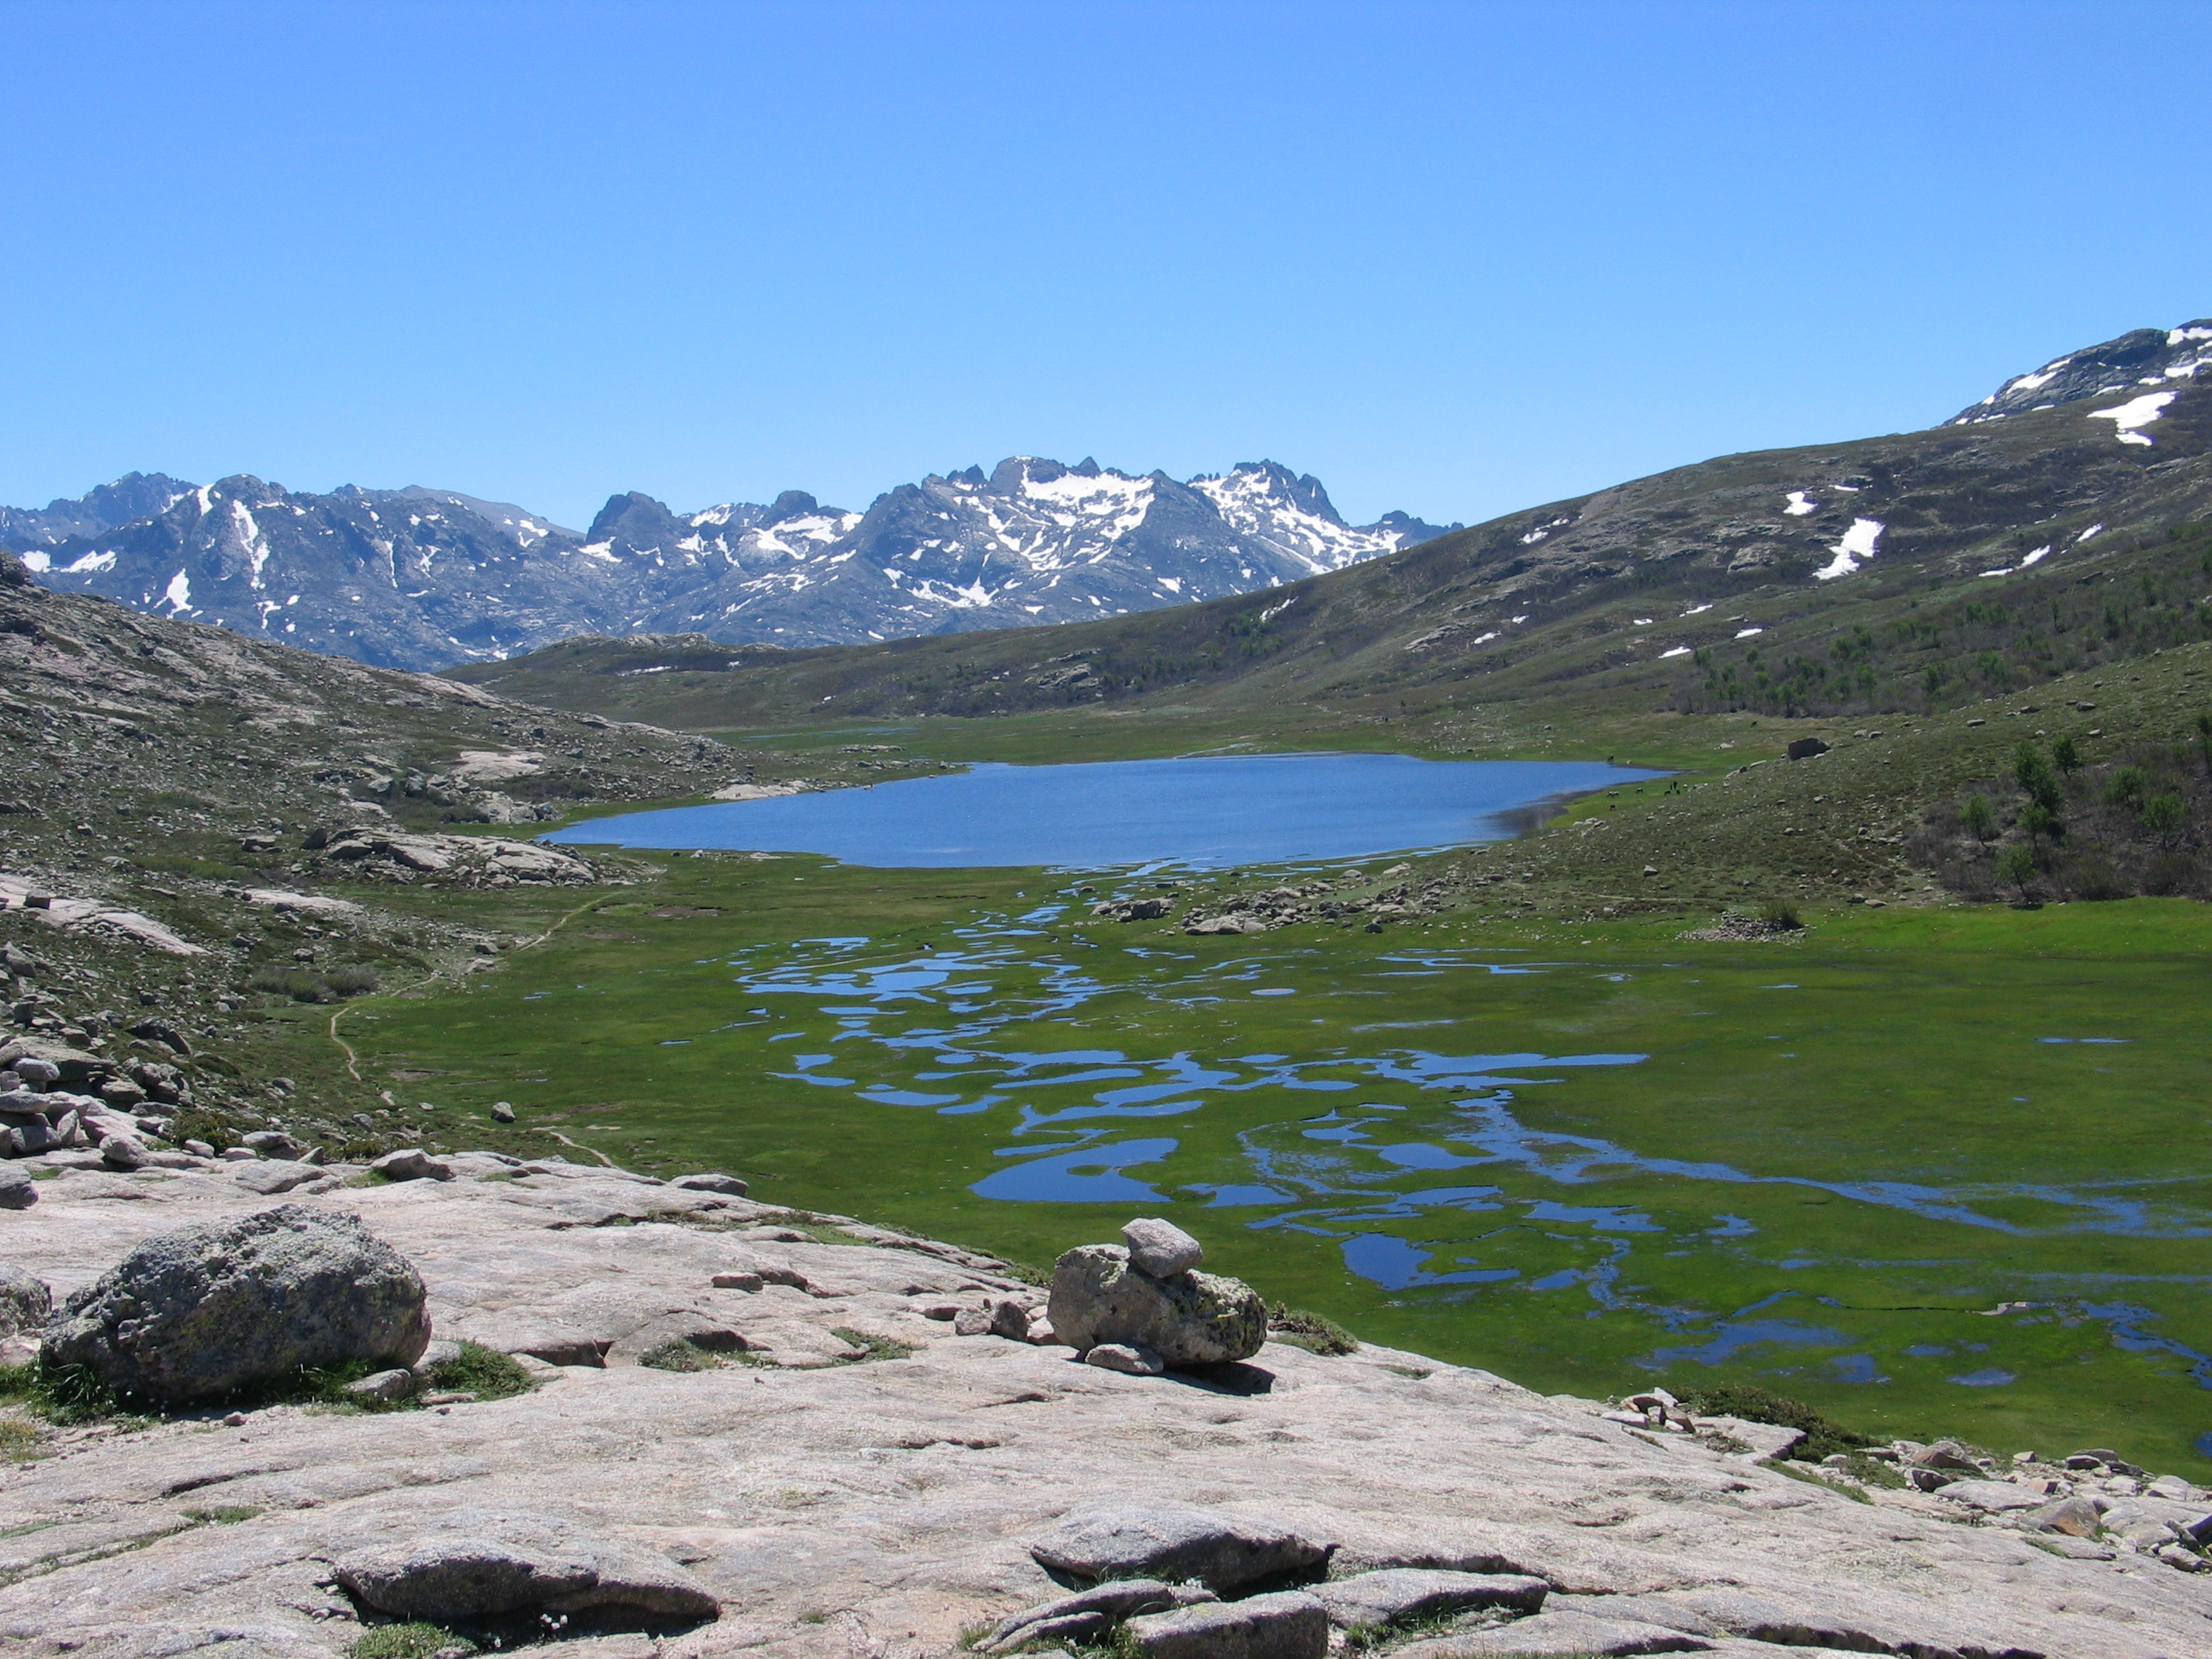
\includegraphics[width=\linewidth]{Lac_de_Nino}
		\caption[Lac de Nino]{Exemple d'image comportant plusieurs éléments notables tels qu'un lac (bleu sombre et uniforme), une plaine herbeuse (verte et uniforme), d'éléments rocailleux qui sont gris et soit uniformes (dans le premier plan) soit plus contrastés en se combinant avec la verdure de la végétation (dans les bords de l'image), et ainsi de suite.[Modifier la figure]}\label{fig:img:nino}
	\end{figureth}

	\subsection{Apprentissage et reconstruction}\label{sec:img:compression}
	\subsubsection{Apprentissage}
	La première étape nécessaire à l'apprentissage est la constitution de la base d'apprentissage à partir de l'image. L'utilisation de modèles de quantification vectorielle établissent la première contrainte pour le découpage : les imagettes doivent être d'une taille fixe. En effet il est nécessaire pour les SOM comme pour les GNG et leurs variantes que tous les vecteurs d'entrées soient de la même longueur pour que le calcul de distance avec les neurones fonctione, qu'ils représentent le plus fidèlement possible les entrées qui leurs sont attachées.

	Nous avons également choisi de limiter nos tailles d'imagettes à des carrés, avec la hauteur égale à la longeur, pour des raisons de simplicité. Il est possible que des imagettes plus larges que hautes ou plus hautes que larges représentent mieux les éléments de l'image que l'on apprend. Cependant ce serait une préférence spécifique à chaque image et peu généralisable, car si on effectue par exemple une rotation de 90° de l'image, la préférence s'inversera. L'inversement des tailles dans les imagettes carrées ne changeant rien, elles sont pour leur part insensibles aux rotations discrètes de l'image (par pas de 90°).

	Dans la version classique \cite{amerijckx-compression}, le découpage de l'image se fait en mosaique, sans superpositions entre les imagettes. C'est à dire que chaque pixel n'appartient qu'à une seule imagette. Le processus est montré sur la figure \ref{fig:img:rep} Si les dimensions de l'images ne sont pas un multiple de la taille des imagettes, les pixels en trop sont rognés par la droite et par le bas [possible de centrer et de rogner tous les côtés en même temps], car en général les bords ne contiennent pas beaucoup d'informations.

	\begin{figureth}
		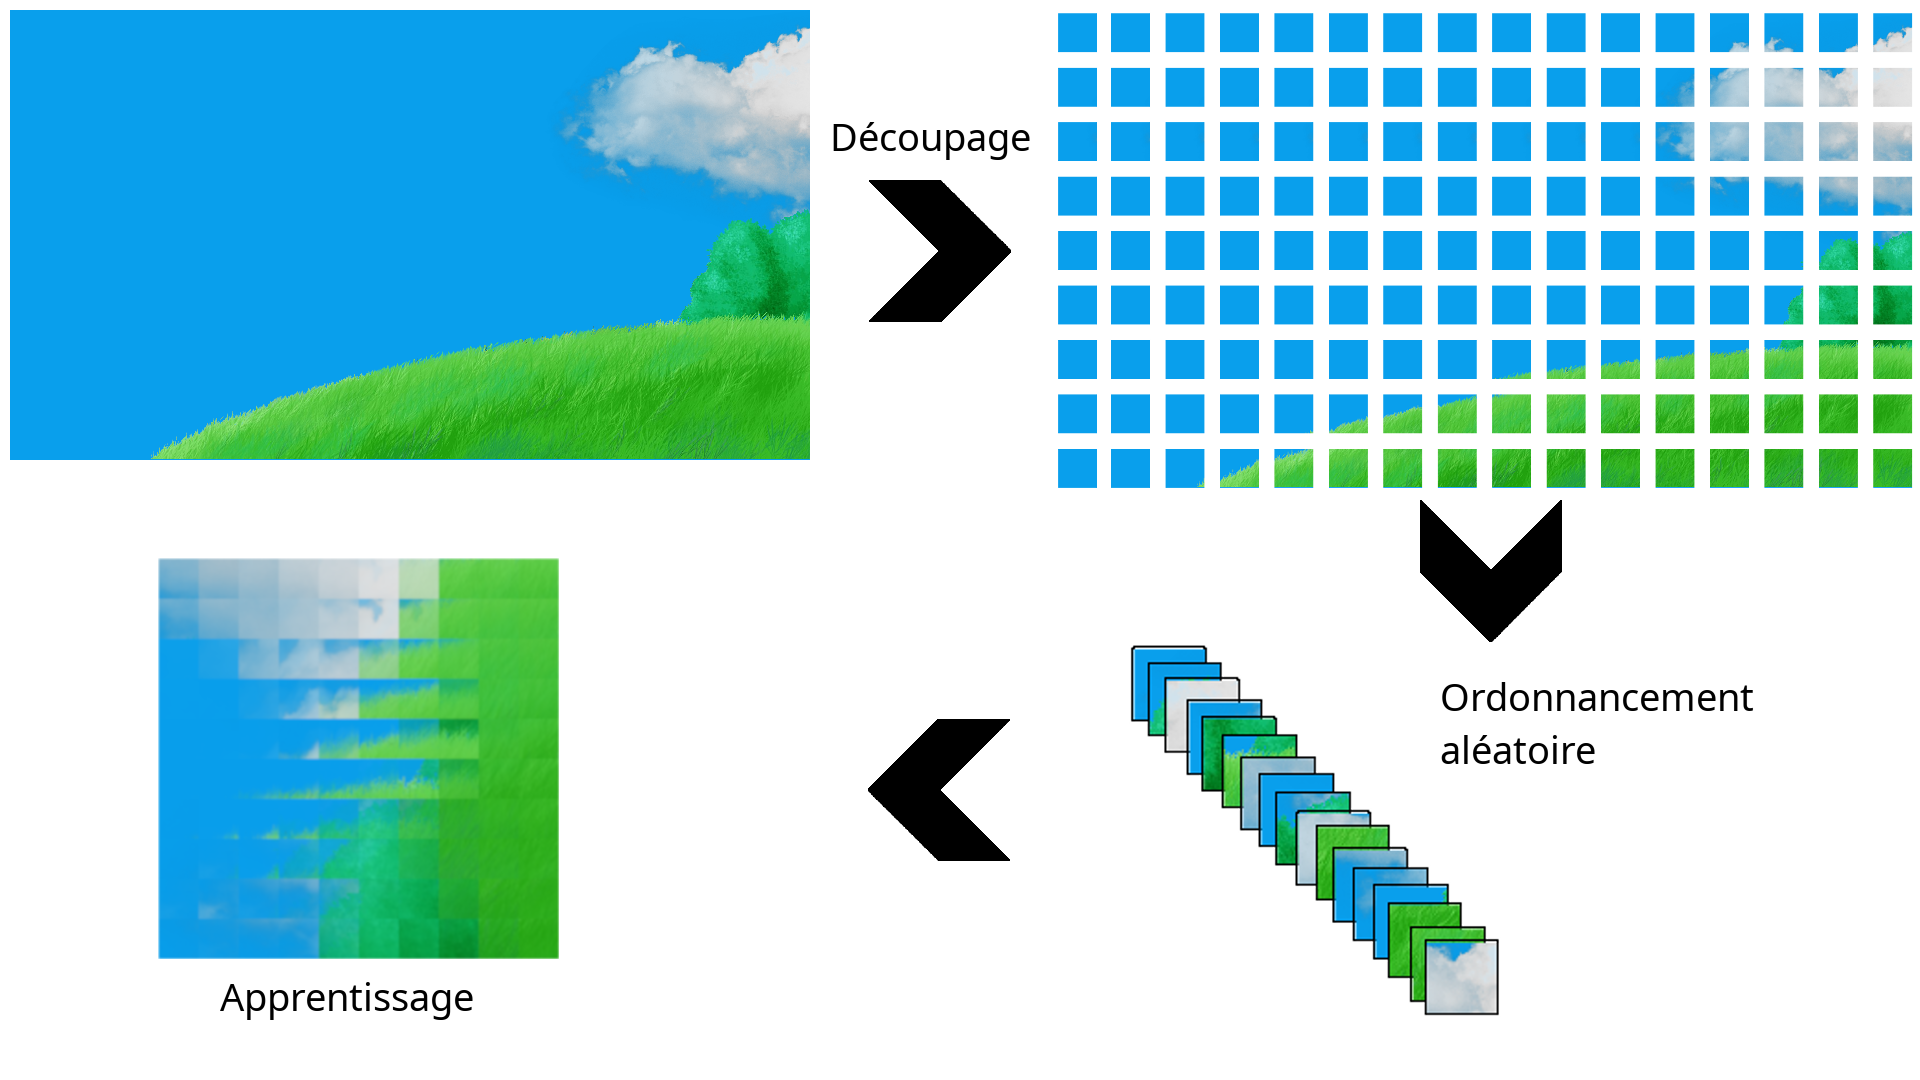
\includegraphics[width=\linewidth]{image_representation}
		\caption[Représentation d'une image]{Illustration du processus de représentation et d'apprentissage d'une image par une SOM.}\label{fig:img:rep}
	\end{figureth}

	\subsubsection{Reconstruction}

	Une fois l'apprentissage terminé, il y a deux résultats. Le premier est le modèle entrainé avec les différents poids des neurones codant une imagette représentante du cluster d'imagettes associé à ce neurone. Le second est la liste pour chaque imagette de l'image l'indexe du neurone le plus proche de celle-ci, qui pourra être utilisée pour la reconstruction de l'image d'apprentissage.  

	Pour reconstruire une image à partir de la liste des indexes de BMU, il suffit de remplacer chaque index par le vecteur prototype du neurone auquel il correspond. Ces vecteurs prototypes devront être réassemblés en imagettes (dans un tableau à 2 dimensions à la place d'un vecteur à une dimension), et placées à la bonne position pour reformer l'image.

	Il est aussi possible de reconstruire une image qui n'a pas été apprise. Pour cela il faut créer la liste d'indexes de neurones des imagettes de la nouvelle image, et de reconstruire ensuite l'image par le même procédé que montré précédemment. Il faut noter que l'image que l'on souhaite reconstituer doit être proche de l'image apprise pour obtenir un résultat correct.

	\begin{figureth}
		\begin{subfigureth}{\textwidth}
			\includegraphics[width=\linewidth]{triangle/Image_compression2}
		\end{subfigureth}
		\begin{subfigureth}{\textwidth}
			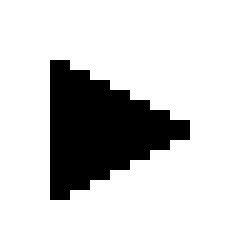
\includegraphics[width=0.2\linewidth]{triangle/triangle_original}\hfill
			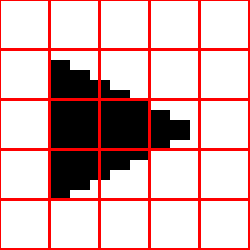
\includegraphics[width=0.2\linewidth]{triangle/triangle_grid}\hfill
			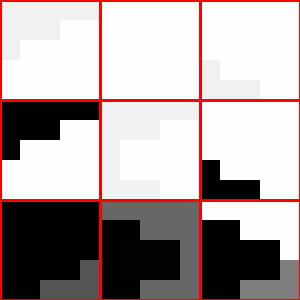
\includegraphics[width=0.2\linewidth]{triangle/som}\hfill
			
\includegraphics[width=0.2\linewidth]{triangle/triangle}
		\end{subfigureth}
		\caption[Compression et décompression d'image]{Schéma simplifié du processus de compression et de reconstruction d'une image, avec ici seulement 9 neurones et 25 imagettes.}\label{fig:img:comp_ex}
	\end{figureth}

	\subsection{La gestion des canaux (couleurs)}\label{sec:img:colors}

	Nous avons jusque là vu comment apprendre une image ayant une seule valeur par pixel (soit des images en nuances de gris). Cependant la majorité des dispositifs de capture actuels fournissent des images en couleur, c'est à dire trois canaux. Nous allons voir dans cette section comment transposer l'apprentissage, la compression et la reconstruction à des images à un nombre arbitraire de canaux par pixels.

	Une approche possible serait de séparer l'image par composante. Une image RVB par exemple donnerait trois images en niveau de gris, une R, une V et une B. Deux options s'offrent ensuite à nous. Soit utiliser une seule SOM pour apprendre toutes les images ainsi extraites en espérant que les différentes formes présentes dans chaque composante soient assez similaires entre elles. Cela augmente aussi les données que la SOM doit apprendre, car on vient de multiplier la taille de notre base d'apprentissage par le nombre de canaux. Ces données doivent être aussi cohérentes dans l'espace d'entrée pour que la réduction dimensionnelle se fasse correctement. Soit utiliser une SOM par composante pour apprendre chaque canal séparément, et de regrouper ensuite les différents canaux reconstitués en une image couleur. 
	
	Cependant ces deux approches ont un défaut majeur pour la compression d'images (ainsi que la détection de nouveauté par conséquent), c'est la création d'aberrations chromatiques dans l'image reconstituée. En effet, les canaux étant appris séparément avant d'être recombinés, la reconstruction peut donner pour certains pixels des teintes de couleurs qui n'existaient pas dans l'image de base, et très saillants visuellement. Par exemple un pixel blanc dans l'image d'entrée (avec une forte composante R, V et B), lorsque reconstitué par la SOM peut être bien reconstitué dans deux composantes (V et B par exemple), et mal reconstitué dans la troisième (R) avec une valeur beaucoup plus faible que dans l'image de base (cela arrive car notre calcul de distance minimise ). Par conséquent ce pixel aura une couleur turquoise dans l'image reconstituée à la place de blanc. Cette erreur minimise bien la distance avec l'image de base, et ce n'est que visuellement que les changements de teintes sont apparents et dégradent proportionnellement plus la qualité de l'image que que l'erreur mesurée.

	Une meilleure approche consiste à inclure tous les canaux directements dans les imagettes. Chaque imagette devient donc une imagette en couleur, et sa taille augmente donc en conséquence. Une imagette de 10 par 10 pixels par exemple qui donnerait un vecteur prototype de taille 100, passe à 300 avec les trois couleurs. L'apprentissage et la reconstruction se déroulent de la même manière que dans la SOM classique. Il faut aussi noter que l'ordre n'a pas d'importance dans les vecteurs prototypes, on peut arranger les valeurs en RGBRGBRGB tout comme RRRGGGBBB sans que cela ne change le résultat, le calcul de distance euclidienne étant indépendant de l'ordre des coordonnées.

	\begin{figureth}
		\begin{subfigureth}{0.48\textwidth}
			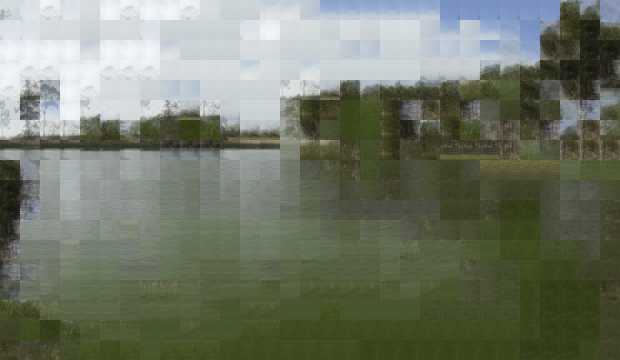
\includegraphics[width=\linewidth]{fusioned_color}\caption{Couleurs fusionnées}	
		\end{subfigureth}
		\begin{subfigureth}{0.48\textwidth}
			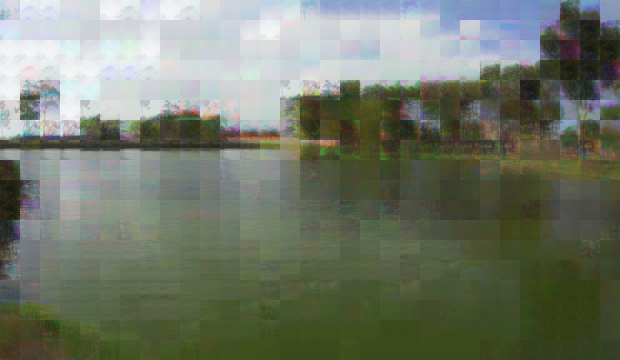
\includegraphics[width=\linewidth]{separated_colors}\caption{Couleurs séparées}	
		\end{subfigureth}
		\caption[Représentation d'une image]{Comparaison entre une image avec des couleurs fusionnées et la même image avec des couleurs séparées qui présente des artefacts visuels.[Faire un exemple plus visuel]}\label{fig:img:rep}
	\end{figureth}

	\newpage
	\section{Détection de nouveauté}

	Nous avons à partir des différentes propriétés de nos modèles neuronaux développé des processus de détection de nouveauté. Ces processus ne sont pas intrinsèques à nos modèles, c'est à dire que nos modèles neuronaux n'ont pas été définis dans le but d'effectuer une détection de nouveauté. Elle est une propriété émergente de ces modèles. Nous présentons ces deux méthodes dans cette section. La première est basée sur la propriété de quantification vectorielle et la seconde sur la topologie.

	\subsection{Détection avec quantification vectorielle}

	\begin{figureth}
		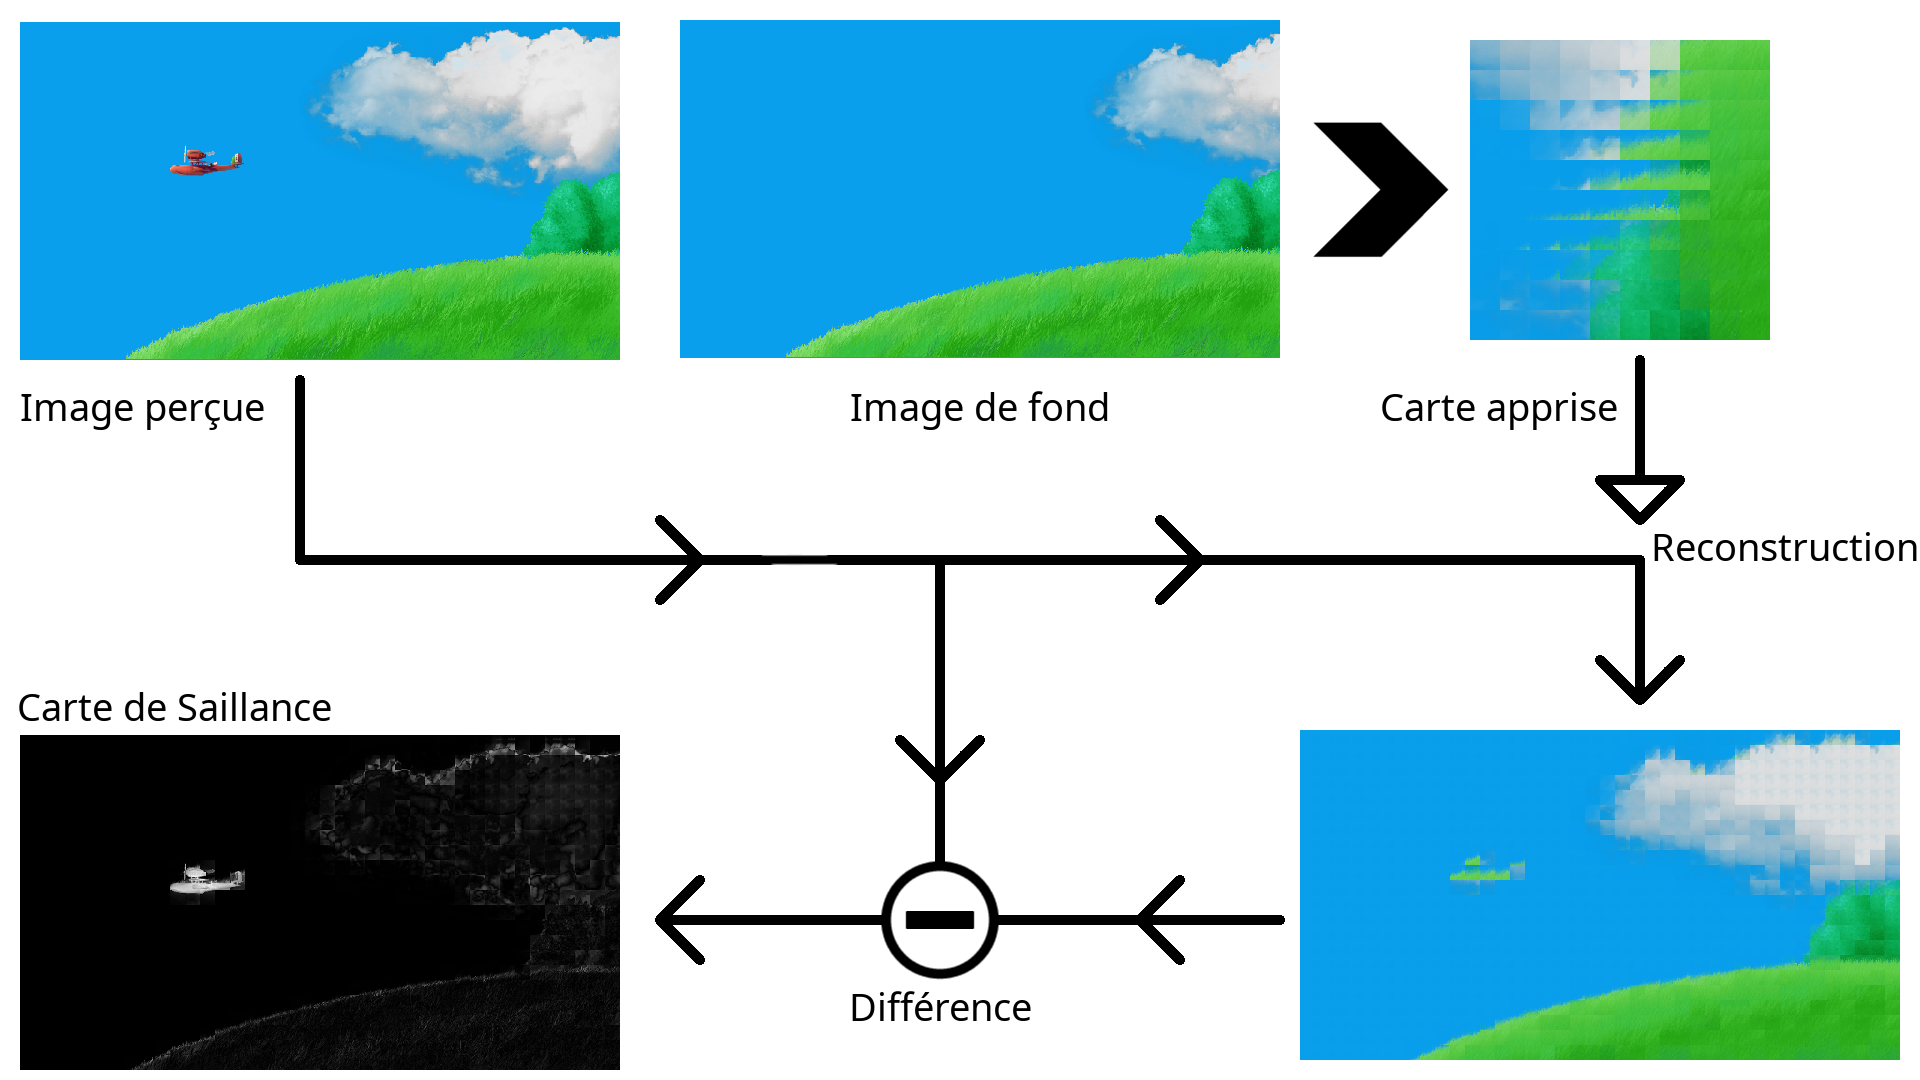
\includegraphics[width=\linewidth]{saliency_map_generation}
		\caption[Détection de nouveauté par quantification vectorielle]{On peut observer qu'il y a eu deux changements entre le fond et l'image perçue : un avion est apparu et les nuages ont bougé. Les nuages, déjà présents dans le fond sont bien reconstruits. L'avion cependant est nouveau, et n'est pas bien reconstruit. Ainsi la différence entre l'image perçue et la reconstruction rend plus saillant l'avion que les nuages. Contrairement à une simple différence entre le fond et l'image perçue, où les deux seraient saillants. Nous avons représenté le modèle appris comme étant une SOM sur cette figure, cependant il peut s'agir de n'importe quel modèle de quantification vectorielle.}\label{fig:img:vq}
	\end{figureth}

	La détection par quantification vectorielle repose sur l'erreur de reconstruction de la nouvelle image provenant du capteur. Cette erreur est la différence entre la nouvelle image et celle reconstruite avec le modèle de VQ ayant effectué son apprentissage sur l'image de fond.

	Il y a deux cas à considérer pour chaque imagette de la nouvelle image du capteur : soit la nouvelle imagette est similaire à une partie quelconque de l'arrière-plan appris, soit quelque chose de nouveau est présent dans l'imagette. Dans le premier cas, le neurone représentatif de cette imagette sera proche de celle-ci, c'est à dire que les poids du neurones et de l'imagette seront proches. L'erreur de reconstuction de cette imagette sera faible, surtout si la caméra est statique, mais avec une petite différence toujours présente en raison des pertes de la compression et des changements naturels de l'environnement visuel.
	
	Cependant, dans le second cas, le neurone représentatif de l'imagette sera éloigné de celle-ci, dans le sens où ses poids seront très différents de ceux de l'imagette. Car la nouveauté est par définition quelque chose qui n'était pas présent dans l'arrière-plan et donc quelque chose que le modèle n'a pas appris. Cela entraînera à une différence significative lors du calcul de la soustraction entre l'image perçue et sa reconstruction à l'endroit de la nouveauté. Ce processus est illustré dans la figure \ref{fig:img:vq}. 

	Ce processus a l'avantage d'être précis au niveau du pixel pour la mise en évidence des changements [Préciser que la taille des imagettes limites quand même la précision]. Il est aussi théoriquement insensible au déplacement d'objets du fond pour la détection de la nouveauté. Cependant, il peut être bruité en raison de l'apprentissage imparfait de la VQ et de la variabilité naturelle de l'environnement.

	\subsection{Détection avec distance neurale}

	\begin{figureth}
		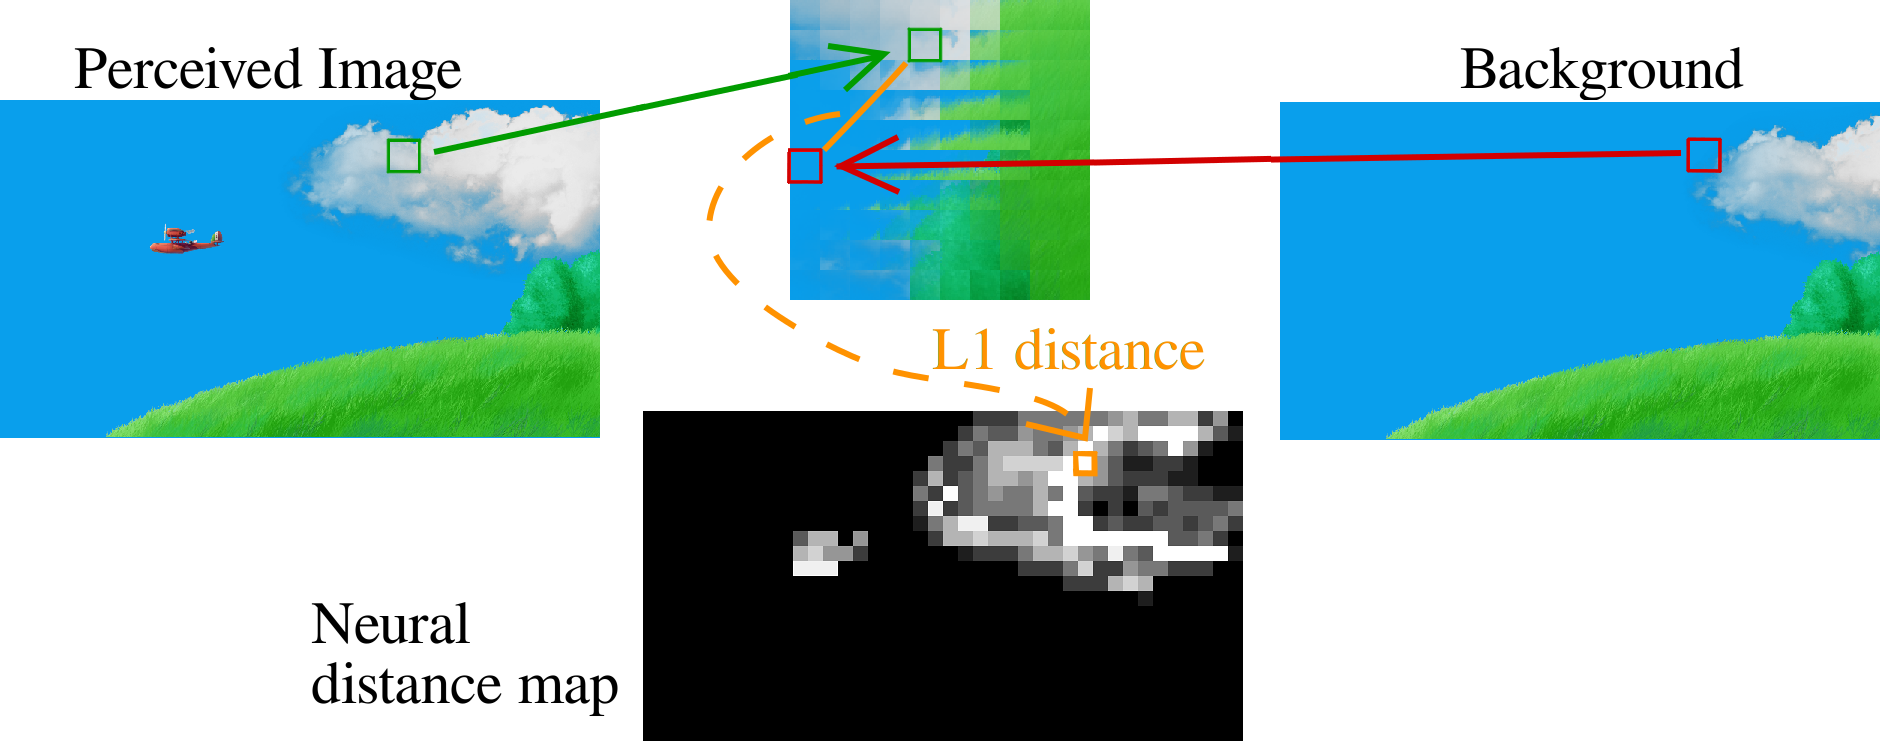
\includegraphics[width=\linewidth]{neural_distance_modulation_v2}
		\caption[Détection de nouveauté avec topologie]{Le processus présenté ici concerne une position dans l'image, et il est répété sur toute l'image pour obtenir la carte de distances neurales en bas. Nous avons représenté le modèle appris comme étant une SOM sur cette figure, cependant il peut s'agir de n'importe quel modèle avec une topologie regroupant les éléments proches.[Traduire la figure en français]}\label{fig:img:topo}
	\end{figureth}

	La détection avec distance neurale se base sur les propriétés topologiques du modèle pour trouver la nouveauté dans une image. La topologie est ce qui relie les différents neurones de modèle par leur proximité : les neurones proches dans la topologie ont appris des poids similaires.

	Après avoir effectué l'apprentissage du modèle, nous mémorisons la liste des positions dans la carte des neurones représentant trouvés pour toutes les imagettes.Lorsqu'une nouvelle image est présentée au capteur, nous effectuons le processus de reconstruction comme dans la première méthode de détection de la nouveauté. Nous nous intéressons uniquement à la liste des positions dans la carte des neurones représentant trouvés pour toutes les imagettes de la nouvelle image. En comparant les deux listes, nous pouvons trouver des changements dans les positions des BMU pour chaque emplacement d'imagette. Si la BMU est la même entre le fond et la nouvelle image à un endroit, alors il n'y a probablement pas de nouveauté à cet endroit. S'il y a une différence entre les deux BMU, alors il pourrait y avoir de la nouveauté à cet endroit. Pour quantifier cette différence, nous calculons la distance topologique qui les sépare sur la carte. La distance topologique est définie par le nombre de nœuds qui sont traversés par le chemin le plus court entre les deux BMU dans la topologie de la carte. Dans la SOM classique basée sur une grille, il s'agit simplement de la distance L1.

	Grâce à ces distances, nous pouvons créer une carte de saillance où des distances élevées dans la topologie signifient des changements significatifs dans l'image, car la proximité dans la topologie signifie la proximité dans l'espace d'entrée. Cette méthode permet d'obtenir une carte de saillance plus robuste, avec moins de bruit que la version avec la VQ. La précision est limitée à la taille des imagettes et il n'y a pas d'inhibition pour les éléments déjà connus qui se sont déplacés dans la fond. Le processus est illustré dans la figure \ref{fig:img:topo}.

	\subsection{Considérations pour la combinaison}
	
	Une fois les deux cartes de saillance générées, il est nécessaire de les combiner pour n'avoir qu'un seul résultat qui représentera la sortie de notre système. Il existe un très grand nombre de façons de le faire cette combinaison, et il existe dans la littérature des modèles qui se basent sur une bonne combinaison de différentes cartes de saillance pour obtenir de meilleurs résultats [citation]. Dans notre cas, nous avons avons préféré utiliser une combinaison simple de nos deux cartes de saillance. C'est à dire qu'elle n'utilise pas de paramètres, pour ne pas ajouter une variable de plus à optimiser. Nous souhaitons aussi bénéficier de la complémentarité des deux cartes de saillances. La solution la plus simple est de multiplier les deux cartes ensemble. Ainsi, sera considéré comme nouveauté dans la carte de sortie, ce qui apparaît comme nouveauté en même temps dans les deux cartes de saillance. Car $\textit{petit} \times \textit{petit} = \textit{petit}$, $\textit{grand} \times \textit{petit} = \textit{petit}$ et seulement $\textit{grand} \times \textit{grand} = \textit{grand}$. Le bruit présent dans la carte résultant de la quantification vectorielle et qui n'est pas présent dans la carte topologique disparaît de la carte finale. Il en va de même pour les mouvements qui ne sont pas des nouveautés qui apparaissent dans la carte topologique, mais pas dans la carte de quantification vectorielle.

	Un problème qui peut apparaître avec cette méthode est la trop petite valeur du résultat et le déséquilibre d'impact de nos deux cartes, car nos cartes de saillance sont toutes les deux définies entre 0 et 1. Il est possible que des situations arrivent lors desquelles les deux cartes ont un impact disproportionnel sur le résultat. Par exemple si la saillance a une valeur de 0.2 sur une carte et 0.8 sur l'autre, alors la seconde aura plus d'impact sur les valeurs de la sortie finale. De même, en multipliant deux nombres compris entre 0 et 1, le résultat sera forcément inférieur à chacun des deux nombres. Cela a un effet réducteur sur toutes les valeurs de la carte de saillance finale. La solution que nous avons choisi à ces deux problèmes, est de re-normaliser les deux cartes de saillances avant de les multiplier. C'est à dire que l'on rééchelonne l'ensemble de la carte en mettant la valeur maximum de la carte à 1 et le minimum à 0 et d'étaler les valeurs intermédiaires entre les deux pour conserver le même espacement relatif entre elles. Cela a pour effet d'éviter une trop grande disproportion d'impact entre les deux cartes sans résoudre complètement le problème cependant. Car on re-normalise avec le maximum, et non avec la possible valeur de la nouveauté detectée. Cela permet également d'avoir un résultat avec des valeurs généralement plus hautes. Cependant, cela vient aussi avec des désavantages, comme par exemple le fait que si il n'y a pas de signal dans l'entrée, le maximum des cartes de saillance sera quand même 1. On pourrait observer des signaux positifs dans la sortie alors que l'entrée et les cartes de saillances n'en montrent pas. En pratique, cela est peu fréquent car la valeur maximum dans un cas où il n'y a pas de signal en entrée vient du bruit, et est donc décorellée entre les deux cartes, et disparaîtra lors de la multiplication. De plus, la taille du signal d'entrée compte, et il est peu probable que du bruit seul puisse créer une zone de signal assez large pour être confondu avec une vraie nouveauté.

	\newpage
	\section{Protocole expérimental}

	Cette section regroupe l'ensemble des considérations pratiques pour la réalisation de nos expériences. Nous présenterons la base de donnée utilisée, comment ces données ont été préparées, les différentes métriques que nous avons mesuré et les paramétrages de nos modèles.

	\subsection{Présentation de la base de données}

	Il n'existe pas à notre connaissance de base de données de détection de nouveauté respectant nos hypothèses de caméra statique, de [...]. Une alternative se trouve dans la base de donnée CDnet \cite{wang-cdnet}. Elle a pour objectif d'uniformiser les résultats dans un domaine proche de la détection de nouveauté ; la détection de changement. Les deux domaines peuvent sembler similaires au premier abord car les deux approches visent la même application réelle. Cependant cela cache une différence conceptuelle. La détection de changement se concentre sur le mouvement pour séparer le fond des objets intéressants dans une image. La détection de nouveauté quand à elle se réfère à une représentation apprise de l'environnement (discuté plus en détail dans la section [...]). Dans les captures vidéos réelles, les deux sont généralement équivalents dû au fait que lorsqu'une nouveauté apparaît, elle le fait généralement en se déplaçant. En pratique cela veut dire que la majorité de CDnet peut être utilisé pour de la détection de nouveauté. Nous présenterons les catégories et vidéos que l'ont a utilisé, et des exemples de vidéos qui n'ont pas été retenues avec des explications dans la suite.
	
	CDnet regroupe 53 séquences vidéos originaires de sources variées. Elles proviennent principalement de caméras de surveillance ou de captures effectuées par des chercheurs pour leur propres besoins. Il n'y a que des captures réelles, sans images synthétiques de scènes intérieures et extérieures. Les vidéos sont toutes en couleur, sauf pour deux catégories \textit{thermal} et \textit{turbulences}, et de résolution assez faible, allant de $320 \times 240$ de $720 \times 486$ pixels. Elles sont groupées en 11 catégories de 4 à 6 vidéos sensées représenter une variété de difficultés que peuvent rencontrer les modèles de détection de changement. Il existe cependant un certain biais dans CDnet, car il est fortement orienté vers de la détection de personnes et de véhicules. Ces catégories sont présentées dans les figures suivantes.

	Parmi les 11 catégories de CDnet, nous avons décidé d'en utiliser 8 complètement, d'utiliser une version réduite pour 2 d'entre elles et d'en enlever une. Les deux catégories réduites sont \textit{Intermittent Object Motion} et \textit{Low framerate}. La réduction consiste à enlever une partie des vidéos qui ne correspondaient pas à notre tâche de ces catégories et de conserver les autres. Une illustration de la différence entre la détection de changements et la détection de nouveauté qui est la source de la suppression est montré sur la figure \ref{fig:cdnet:diff}. La catégorie que nous avons décidé de ne pas du tout utiliser car elle ne correspondait pas à notre scénario est \textit{Pan tilt zoom}. C'est une catégorie un peu spéciale car elle change une partie fondamentale du scénario. La caméra n'est plus statique mais effectue des roations et des zooms ce qui change significativement son environnement visuel.


	\begin{figureth}
		\begin{subfigureth}{0.24\textwidth}
			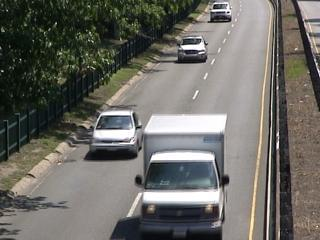
\includegraphics[width=\linewidth]{CDNET/baseline/in000277}\caption{Highway}	
		\end{subfigureth}
		\begin{subfigureth}{0.24\textwidth}
			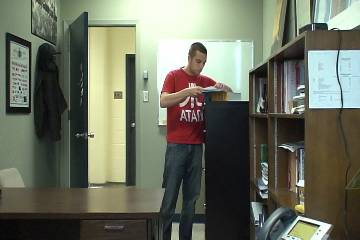
\includegraphics[width=\linewidth]{CDNET/baseline/in000895}\caption{Office}	
		\end{subfigureth}
		\begin{subfigureth}{0.24\textwidth}
			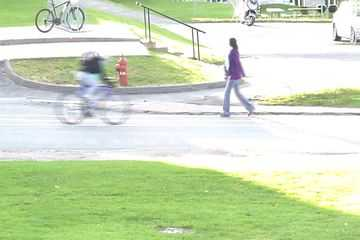
\includegraphics[width=\linewidth]{CDNET/baseline/in000473}\caption{Pedestrians}	
		\end{subfigureth}
		\begin{subfigureth}{0.24\textwidth}
			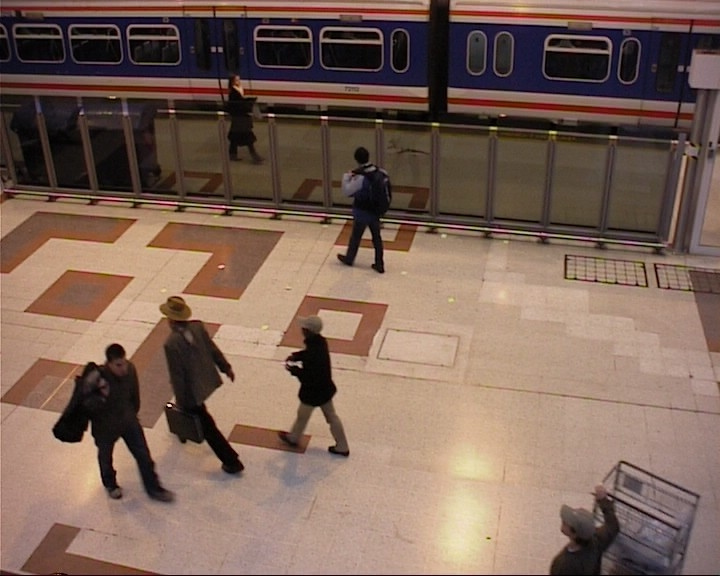
\includegraphics[width=\linewidth]{CDNET/baseline/in000118}\caption{PETS2006}	
		\end{subfigureth}
		\caption[Catégorie Baseline]{\textit{Baseline} : La catégorie de base qui comprend des scénarios typiques de détection de changement (traffic, piétons) sans difficultés particulières.}\label{fig:cdnet:baseline}
	\end{figureth}

	\begin{figureth}
		\begin{subfigureth}{0.24\textwidth}
			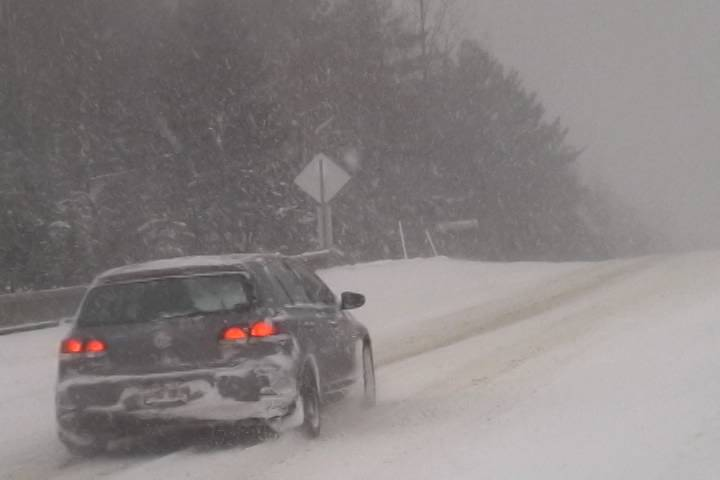
\includegraphics[width=\linewidth]{CDNET/badWeather/in000810}\caption{Snowfall}	
		\end{subfigureth}
		\begin{subfigureth}{0.24\textwidth}
			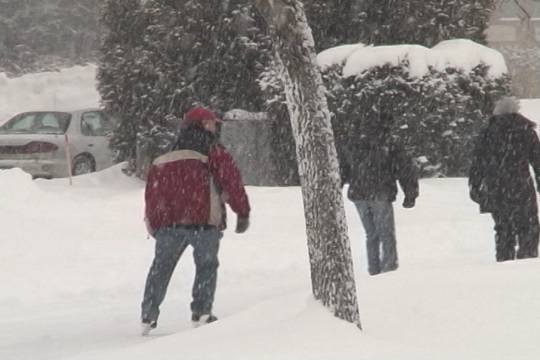
\includegraphics[width=\linewidth]{CDNET/badWeather/in001951}\caption{Skating}	
		\end{subfigureth}
		\begin{subfigureth}{0.24\textwidth}
			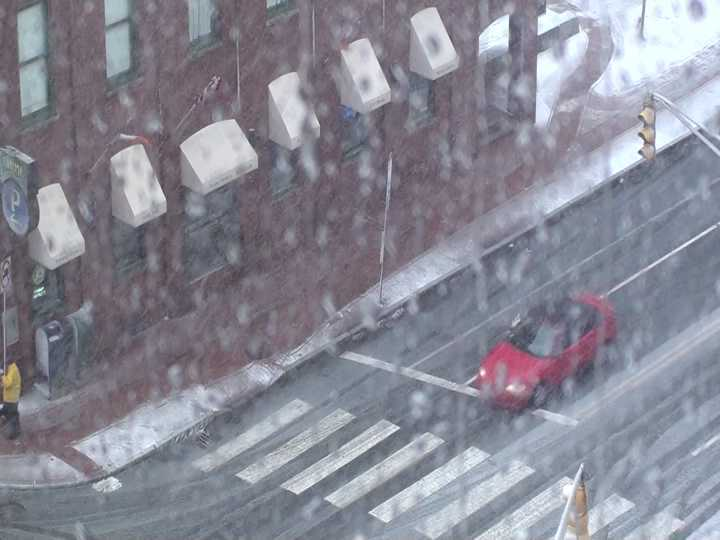
\includegraphics[width=\linewidth]{CDNET/badWeather/in002841}\caption{WetSnow}	
		\end{subfigureth}
		\begin{subfigureth}{0.24\textwidth}
			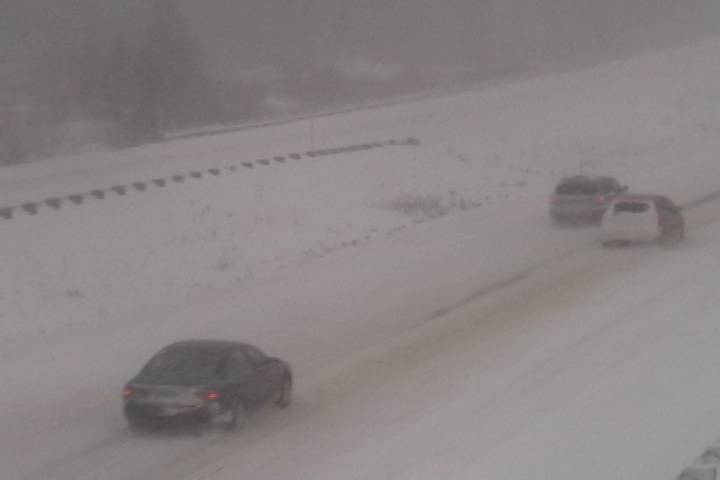
\includegraphics[width=\linewidth]{CDNET/badWeather/in004863}\caption{Blizzard}	
		\end{subfigureth}
		\caption[Catégorie Bad weather]{\textit{Bad weather} : Cette catégorie comprend des variations du scénario de base avec une météo dégradée. La difficulté principale vient de la neige qui tombe, et du changment de l'environnement avec les traces de pneus sur la neige par exemple.}\label{fig:cdnet:badweather}
	\end{figureth}

	\begin{figureth}
		\begin{subfigureth}{0.24\textwidth}
			\includegraphics[width=\linewidth]{CDNET/cameraJitter/in000145}\caption{Sidewalk}	
		\end{subfigureth}
		\begin{subfigureth}{0.24\textwidth}
			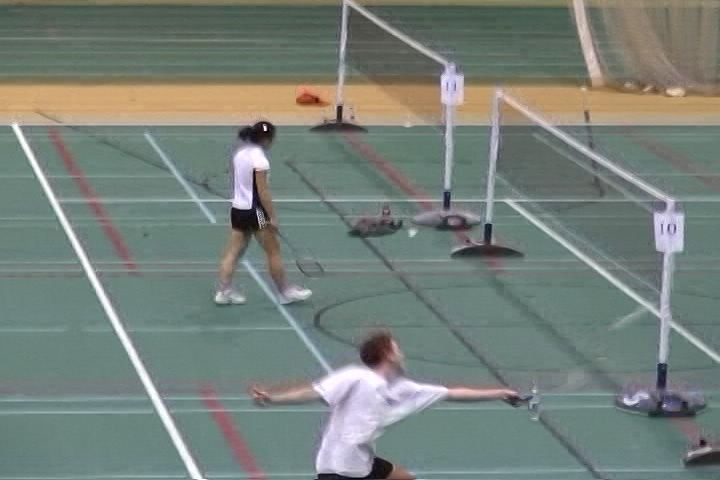
\includegraphics[width=\linewidth]{CDNET/cameraJitter/in000187}\caption{Badminton}	
		\end{subfigureth}
		\begin{subfigureth}{0.24\textwidth}
			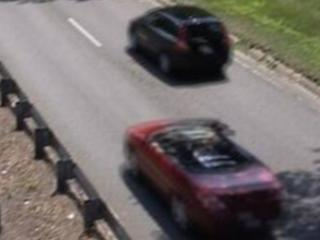
\includegraphics[width=\linewidth]{CDNET/cameraJitter/in000355}\caption{Traffic}	
		\end{subfigureth}
		\begin{subfigureth}{0.24\textwidth}
			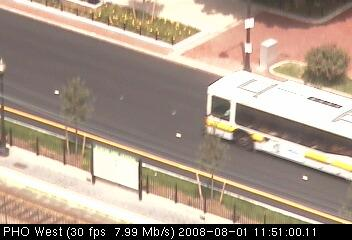
\includegraphics[width=\linewidth]{CDNET/cameraJitter/in002287}\caption{Boulevard}	
		\end{subfigureth}
		\caption[categorie camera jitter]{\textit{Camera Jitter} : Ces vidéos proviennent de caméras instables à cause de vent fort ou d'autres raisons. Elles ont de façon irrégulière des translations verticales et horizontales  rapides et de petite amplitude.}\label{fig:cdnet:jitter}
	\end{figureth}

	\begin{figureth}
		\begin{subfigureth}{0.24\textwidth}
			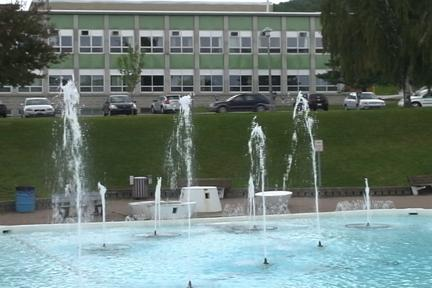
\includegraphics[width=\linewidth]{CDNET/dynamicBackground/in000716}\caption{Fountain01}	
		\end{subfigureth}
		\begin{subfigureth}{0.24\textwidth}
			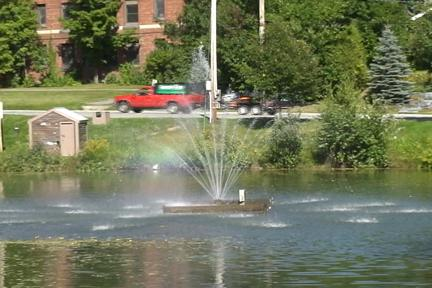
\includegraphics[width=\linewidth]{CDNET/dynamicBackground/in000720}\caption{Fountain02}	
		\end{subfigureth}
		\begin{subfigureth}{0.24\textwidth}
			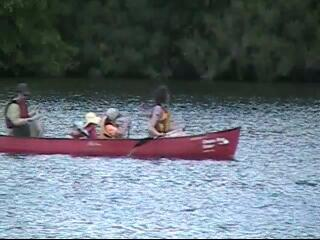
\includegraphics[width=\linewidth]{CDNET/dynamicBackground/in000937}\caption{Canoe}	
		\end{subfigureth}\\
		\begin{subfigureth}{0.24\textwidth}
			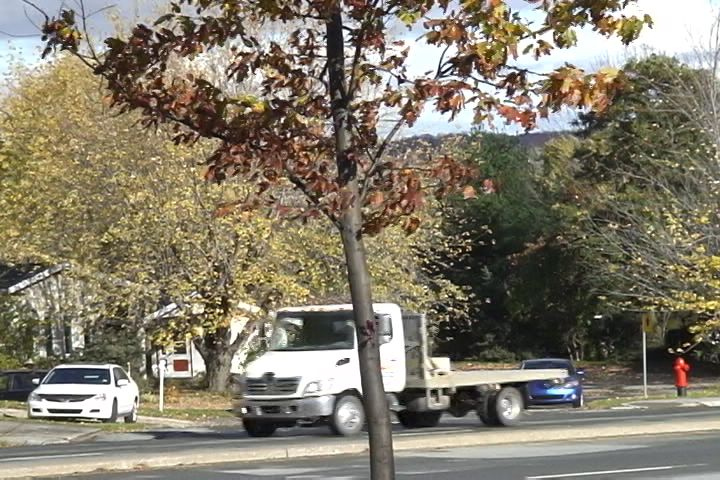
\includegraphics[width=\linewidth]{CDNET/dynamicBackground/in001504}\caption{Fall}	
		\end{subfigureth}
		\begin{subfigureth}{0.24\textwidth}
			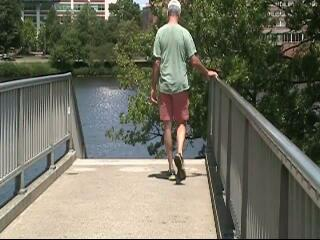
\includegraphics[width=\linewidth]{CDNET/dynamicBackground/in002519}\caption{Overpass}	
		\end{subfigureth}
		\begin{subfigureth}{0.24\textwidth}
			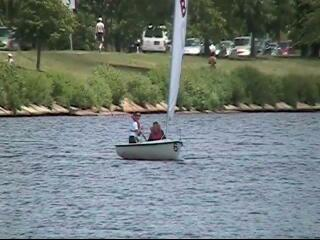
\includegraphics[width=\linewidth]{CDNET/dynamicBackground/in007726}\caption{Boats}	
		\end{subfigureth}
		\caption[Categorie Dynamic Background]{\textit{Dynamic Background} : La difficulté se porte sur le contenu du fond qui est changeant. Il peut s'agir d'eau ou d'arbres qui bougent dans le vent.}\label{fig:cdnet:dynamic}
	\end{figureth}

	\begin{figureth}
		\begin{subfigureth}{0.24\textwidth}
			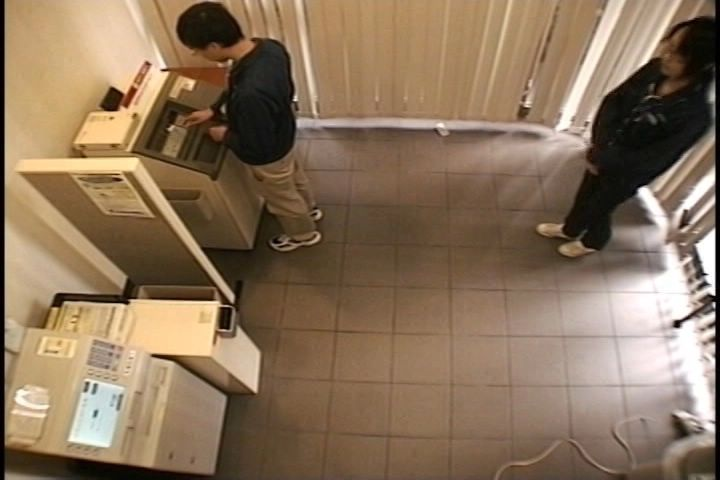
\includegraphics[width=\linewidth]{CDNET/shadow/in000260}\caption{CopyMachine}
		\end{subfigureth}
		\begin{subfigureth}{0.24\textwidth}
			\includegraphics[width=\linewidth]{CDNET/shadow/in000320}\caption{PeopleInShade}
		\end{subfigureth}
		\begin{subfigureth}{0.24\textwidth}
			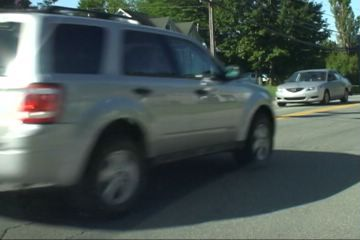
\includegraphics[width=\linewidth]{CDNET/shadow/in000358}\caption{Bungalows}	
		\end{subfigureth}\\
		\begin{subfigureth}{0.24\textwidth}
			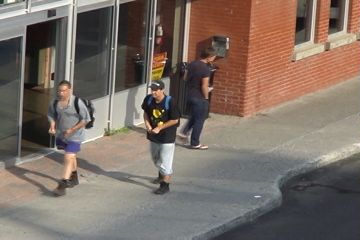
\includegraphics[width=\linewidth]{CDNET/shadow/in001015}\caption{BusStation}	
		\end{subfigureth}
		\begin{subfigureth}{0.24\textwidth}
			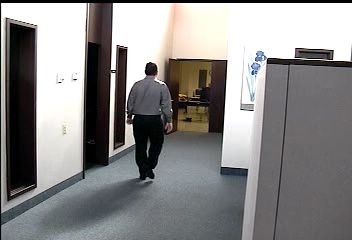
\includegraphics[width=\linewidth]{CDNET/shadow/in001210}\caption{Cubicle}
		\end{subfigureth}
		\begin{subfigureth}{0.24\textwidth}
			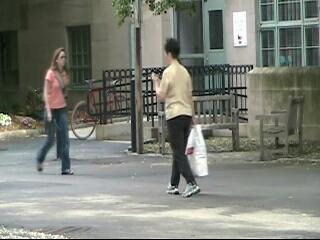
\includegraphics[width=\linewidth]{CDNET/shadow/in001850}\caption{Backdoor}	
		\end{subfigureth}
		\caption[Categorie Shadow]{\textit{Shadow} : Catégorie de vidéos qui présente plus d'ombres que la moyenne.}\label{fig:cdnet:shadow}
	\end{figureth}

	\begin{figureth}
		\begin{subfigureth}{0.24\textwidth}
			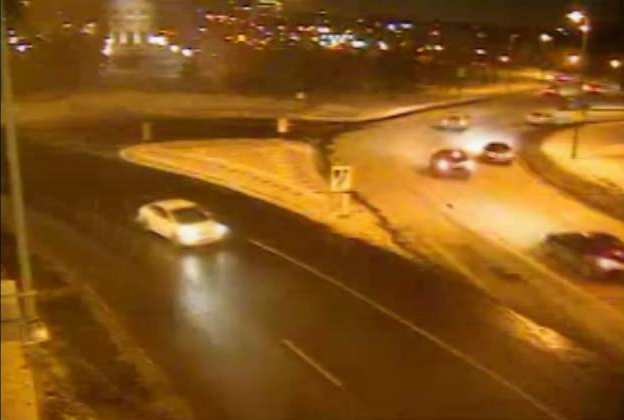
\includegraphics[width=\linewidth]{CDNET/nightVideos/in000060}\caption{WinterStreet}	
		\end{subfigureth}
		\begin{subfigureth}{0.24\textwidth}
			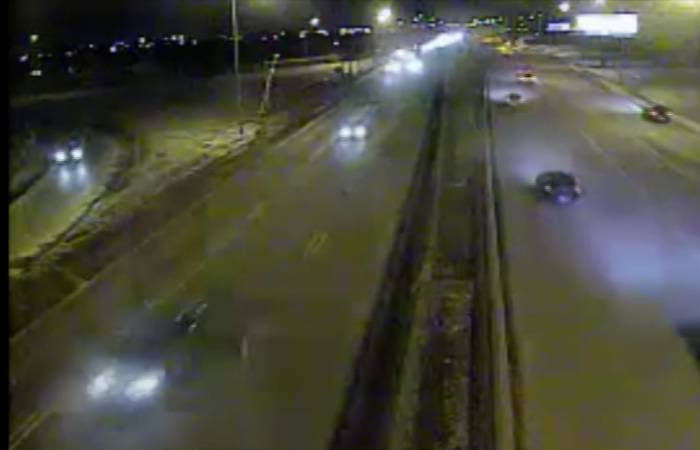
\includegraphics[width=\linewidth]{CDNET/nightVideos/in000125}\caption{FluidHighway}	
		\end{subfigureth}
		\begin{subfigureth}{0.24\textwidth}
			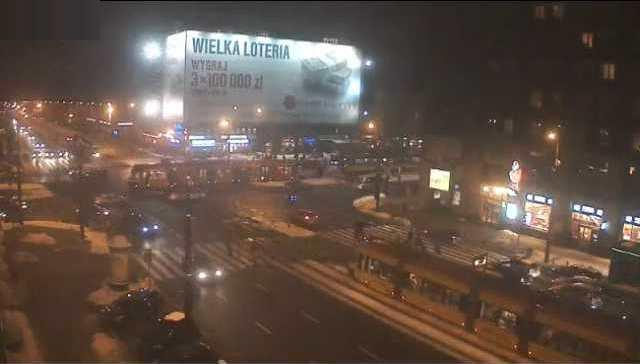
\includegraphics[width=\linewidth]{CDNET/nightVideos/in000150}\caption{BusyBoulevard}	
		\end{subfigureth}\\
		\begin{subfigureth}{0.24\textwidth}
			\includegraphics[width=\linewidth]{CDNET/nightVideos/in000320}\caption{TramStation}	
		\end{subfigureth}
		\begin{subfigureth}{0.24\textwidth}
			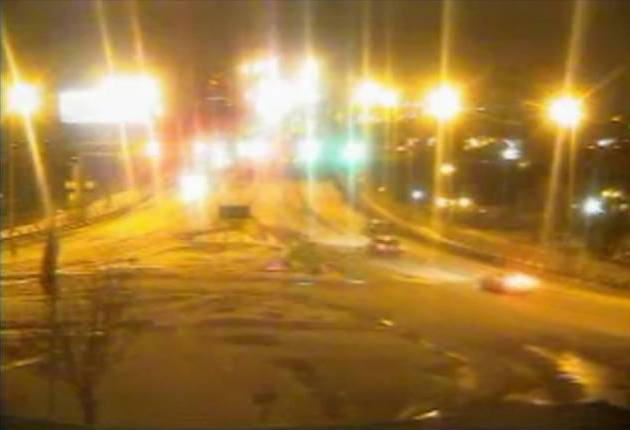
\includegraphics[width=\linewidth]{CDNET/nightVideos/in000362}\caption{BridgeEntry}	
		\end{subfigureth}
		\begin{subfigureth}{0.24\textwidth}
			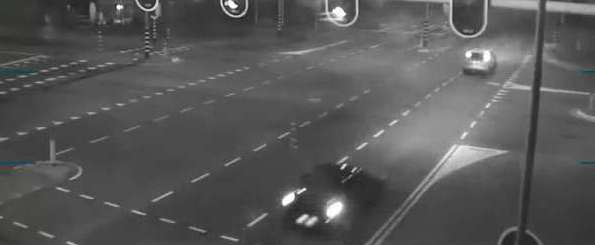
\includegraphics[width=\linewidth]{CDNET/nightVideos/in000671}\caption{StreetCornerAtNight}	
		\end{subfigureth}
		\caption[Categorie Night Videos]{\textit{Night Videos} : Vidéos de nuit avec un contraste fort entre l'obscurité ambiante et les lumières artificielles de l'éclairage public et des phares de voitures.}\label{fig:cdnet:night}
	\end{figureth}

	\begin{figureth}
		\begin{subfigureth}{0.24\textwidth}
			\includegraphics[width=\linewidth]{CDNET/thermal/in000145}\caption{Park}
		\end{subfigureth}
		\begin{subfigureth}{0.24\textwidth}
			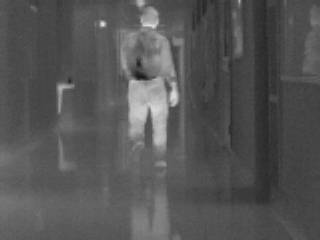
\includegraphics[width=\linewidth]{CDNET/thermal/in000800}\caption{Corridor}	
		\end{subfigureth}
		\begin{subfigureth}{0.24\textwidth}
			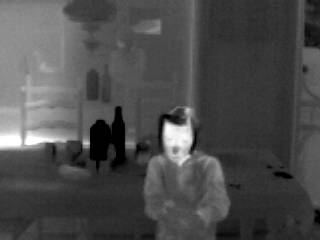
\includegraphics[width=\linewidth]{CDNET/thermal/in000840}\caption{DiningRoom}	
		\end{subfigureth}\\
		\begin{subfigureth}{0.24\textwidth}
			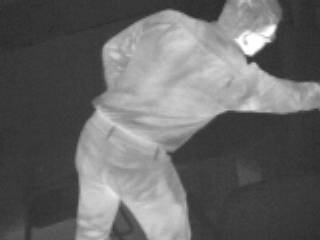
\includegraphics[width=\linewidth]{CDNET/thermal/in001050}\caption{Library}	
		\end{subfigureth}
		\begin{subfigureth}{0.24\textwidth}
			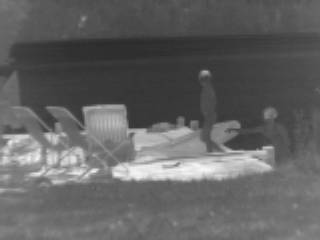
\includegraphics[width=\linewidth]{CDNET/thermal/in002220}\caption{LakeSide}	
		\end{subfigureth}
		\caption[Categorie thermal]{\textit{Thermal} : Ces vidéos ont été prises par une caméra infrarouge et sont en niveau de gris.}\label{fig:cdnet:shadow}
	\end{figureth}

	\begin{figureth}
		\begin{subfigureth}{0.24\textwidth}
			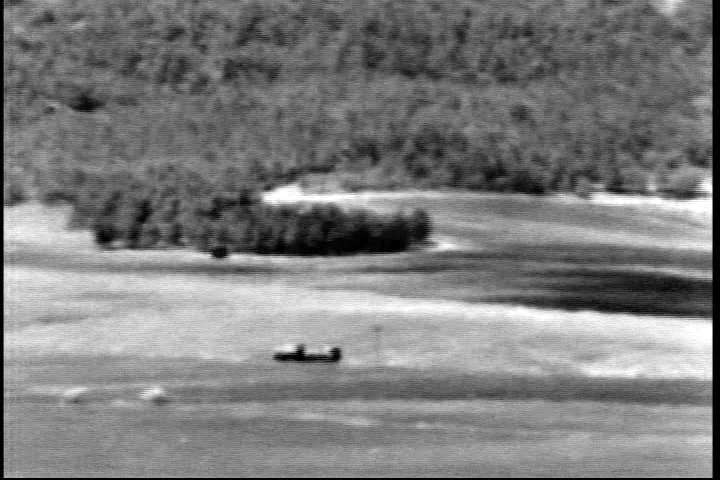
\includegraphics[width=\linewidth]{CDNET/turbulence/in000425}\caption{Turbulence0}	
		\end{subfigureth}
		\begin{subfigureth}{0.24\textwidth}
			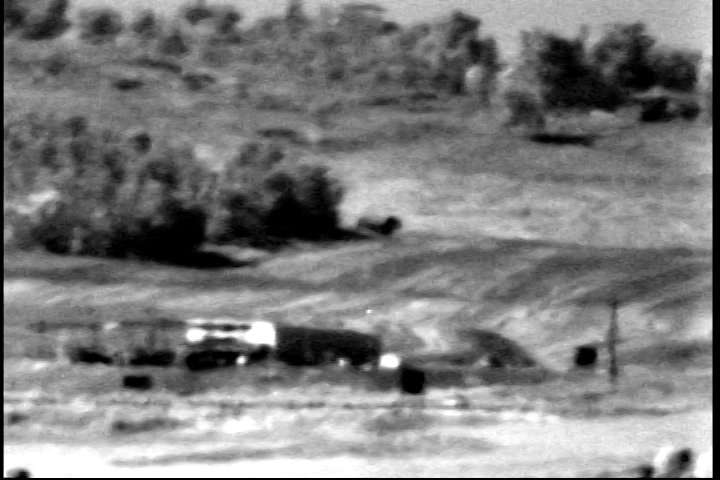
\includegraphics[width=\linewidth]{CDNET/turbulence/in000920}\caption{Turbulence1}	
		\end{subfigureth}
		\begin{subfigureth}{0.24\textwidth}
			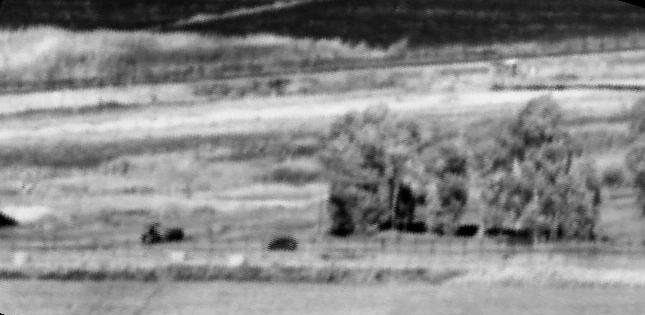
\includegraphics[width=\linewidth]{CDNET/turbulence/in000140}\caption{Turbulence2}	
		\end{subfigureth}
		\begin{subfigureth}{0.24\textwidth}
			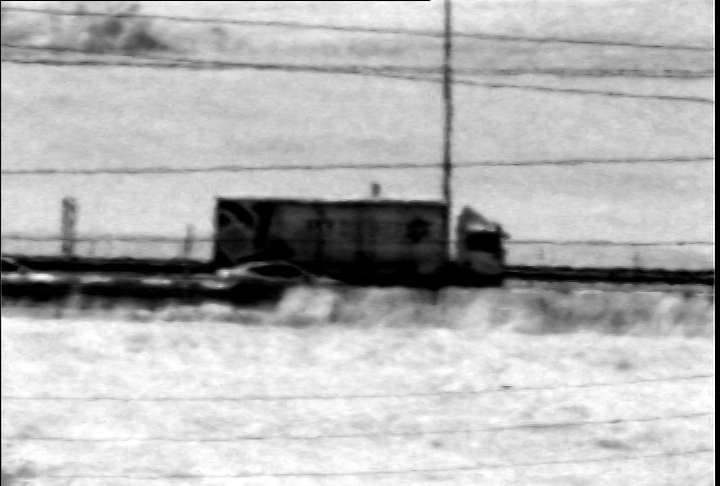
\includegraphics[width=\linewidth]{CDNET/turbulence/in000195}\caption{Turbulence3}	
		\end{subfigureth}
		\caption[Categorie turbulence]{\textit{Turbulence} : Catégorie qui regroupe des vidéos provenant d'une même caméra infrarouge. Les captures ont été faites avec un objectif longue distance filmant des scènes à 5 à 15 km de l'objectif. Elle présente de nombreuses distortions et turbulences atmosphérique dûs à la chaleur et à la distance.}\label{fig:cdnet:turbulence}
	\end{figureth}
	
	\begin{figureth}
		\begin{subfigureth}{0.24\textwidth}
			\includegraphics[width=\linewidth]{CDNET/intermittentObjectMotion/in001000}\caption{StreetLight}
		\end{subfigureth}
		\begin{subfigureth}{0.24\textwidth}
			\includegraphics[width=\linewidth]{CDNET/intermittentObjectMotion/in001300}\caption{Sofa}	
		\end{subfigureth}
		\begin{subfigureth}{0.24\textwidth}
			\includegraphics[width=\linewidth]{CDNET/intermittentObjectMotion/in001350}\caption{Tramstop}	
		\end{subfigureth}
		\caption[Categorie intermittent object motion - Reduced]{\textit{Intermittent object motion Reduced} : Cette catégorie comprend des scénarios particuliers dans lesquels le changement est intermittent (c'est à dire qu'un objet passe de mouvement à statique ou inversement). Dans cette catégorie trois vidéos sur six on été conservées.}\label{fig:cdnet:shadow}
	\end{figureth}

	\begin{figureth}
		\begin{subfigureth}{0.24\textwidth}
			\includegraphics[width=\linewidth]{CDNET/lowFramerate/in000062}\caption{Turnpike}	
		\end{subfigureth}
		\begin{subfigureth}{0.24\textwidth}
			\includegraphics[width=\linewidth]{CDNET/lowFramerate/in000088}\caption{TramCrossroad}	
		\end{subfigureth}
		\begin{subfigureth}{0.24\textwidth}
			\includegraphics[width=\linewidth]{CDNET/lowFramerate/in000235}\caption{Tunnel Exit}	
		\end{subfigureth}
		\caption[Categorie low framerate - Reduced]{\textit{Low Framerate Reduced} : Cette catégorie regroupe des vidéos avec beaucoup de temps entre les images (entre 1 seconde et 6 secondes entre chaque image). Cela a pour but de pénaliser les approches à partir de flow optique, cependant notre approche n'est pas concernée. Trois vidéos sur les quatre ont été conservées. Seule une vidéo d'une marina a été retirée car la nouveauté (des bateaux) était trop similaire au fond, qui consiste en un grand nombre de bateaux ammarés.}\label{fig:cdnet:fps}
	\end{figureth}

	\begin{figureth}
		\begin{subfigureth}{0.24\textwidth}
			\includegraphics[width=\linewidth]{intermittentObjectExample/in001285}\caption{Voiture statique}	
		\end{subfigureth}
		\begin{subfigureth}{0.24\textwidth}
			\includegraphics[width=\linewidth]{intermittentObjectExample/gt001285}\caption{Vérité terrain}
		\end{subfigureth}
		\begin{subfigureth}{0.24\textwidth}
			\includegraphics[width=\linewidth]{intermittentObjectExample/in001815}\caption{Voiture en mouvement}	
		\end{subfigureth}
		\begin{subfigureth}{0.24\textwidth}
			\includegraphics[width=\linewidth]{intermittentObjectExample/gt001815}\caption{Vérité terrain}	
		\end{subfigureth}
		\caption[Difference entre nouveauté and changement]{Ces images sont extraites d'une vidéo de la catégorie \textit{Intermittent Object Motion} et illustrent la différence entre détection de changement et détection de nouveauté. Pour le changement la voiture fait partie du fond pendant une partie de la vidéo car elle est statique. Elle devient objet à détecter à partir du moment où elle commence à se déplacer. Pour la nouveauté, une telle distinction n'est pas possible. Soit elle fait partie du fond, et dans ce cas, même en mouvement elle ne devrait pas être considérée comme nouveauté. Soit elle ne fait pas partie du fond, et dans ce cas elle sera tout le temps considérée comme nouveauté, même lors de la séquence statique.}\label{fig:cdnet:diff}
	\end{figureth}

	\subsection{Métriques utilisées}

	Nous présenterons dans cette section les différentes métriques que l'on a utilisé pour évaluer nos modèles. Elles peuvent être regroupées en deux grandes catégories, la première est proche des modèles évalués (la SOM et les GNG), et essaye de mesurer la qualité d'apprentissage de ceux-ci. La seconde est plus orienté vers la tâche de détection de nouveauté. Cette deuxième catégorie utilise des métriques définies par CDnet pour comparer les résultats avec d'autres modèles. Celles-ci étant en grand nombre, nous nous sommes limités aux trois plus pertinentes qui sont la précision, le rappel et la f-measure.

	\subsubsection{MQE : Erreur de Quantification Moyenne}

	L'erreur de quantification moyenne (Mean Quantization Error) mesure la qualité de l'apprentissage ou de la reconstruction d'un algorithme de quantification vectorielle. C'est la somme des différences entre tous les vecteurs et leurs représentants, divisée par la dimension et le nombre de vecteurs pour obtenir l'erreur moyenne des composantes.
	
	\begin{equation}
		\text{MQE} = \frac{1}{dn} \sum_{i=0}^{n-1} |v_i - u_i|
	\end{equation}
	[glossaire pour la terminologie mathématique employée]

	Il s'agit d'une mesure simple à calculer et à comprendre. Elle présente néanmoins une mauvaise pondération des différences en pénalisant de la même manière les outliers que des différences diffuses. Par exemple un pixel qui aura un changement maximal (qui passe de noir à blanc par exemple) aura le même impact sur l'erreur que cent pixels qui passent de 0 à 0,01. Pour des images, le premier changement sera visible pour notre oeil, mais pas le second. Nous avons quand même choisi d'utiliser cette mesure dans nos expériences car elle représente le mieux la différence numérique des vecteurs à leurs représentants avant notre interprétation subjective de ces valeurs en images.

	\subsubsection{PSNR : Peak Signal to Noise Ratio}

	Le PSNR est une mesure très présente dans le domaine de la compression d'images \cite{huynh-psnr, korhonen-psnr}. Elle est similaire à la MQE, à la différence qu'il y a un carré à la place de la valeur absolue. D'où le nom de Mean Squared Quantization Error (MSQE) à calculer pour pouvoir obtenir le PSNR.
	
	\begin{equation}
		\text{MSQE} = \frac{1}{dn} \sum_{i=0}^{n-1} (v_i - u_i)^2
	\end{equation}
	\begin{equation}
		\text{PSNR} = 10 \log_{10} (\frac{1}{\text{MSQE}})
	\end{equation}

	Le PSNR est inspiré du domaine du traitement du signal, d'où la terminologie étrange pour de la compression d'image. L'idée est de trouver le ratio de bruit introduit par les pertes de la compression (Noise), avec l'intensité maximale du signal (Peak Signal), qui est la valeur maximum d'un pixel (1 dans notre cas). On peut noter que le PSNR fait passer d'un objectif de minimisation à une maximisation. L'ordre des valeurs reste inchangé et le logarithme ajoute un effet de rendement décroissant. Si on a par exemple trois valeurs de MSQE $x_1$, $y_1$ et $z_1$ avec $x_1 < y_1 < z_1$. $x_1$ sera la meilleure (la plus petite) et $z_1$ la moins bonne (la plus grande). Une fois converties en PSNR, les valeurs seront dans l'ordre suivant : $x_2 > y_2 > z_2$, avec $x_2$ étant toujours la meilleure et $z_2$ toujours la moins bonne, mais pour les raisons inverses cette fois : plus un PSNR est grand, mieux c'est. Un autre changement sera que si les intervalles étaient les même entre les trois valeurs, c'est à dire si $y_1 - x_1 = z_1 - y_1$ alors on aura $y_2 - x_2 < z_2 - y_2$, car le logarithme met plus d'espace deux hautes valeurs de MSQE qu'entre deux petites.

	Nous avons choisi d'utiliser le PSNR à la place de la MSQE car il est beaucoup plus facilement interprétable par des humain. Sa valeur typique étant comprise entre 0 et 100. L'utilisation du carré dans la MSQE entraine une plus grande pénalisation des outliers en comparaison à MQE. Ce n'est quand même pas une mesure objective de la qualité d'une image, car elle ne prend pas en compte certains paramètres comme le voisinage par exemple, qui sont importants dans notre perception humaine [réf biblio]. Puisque l'on utilise la distance quadratique dans nos algorithmes de quantification vectorielle, le PSNR est une métrique intéressante car elle est la valeur que notre algorithme tente de minimiser.
	
	\subsubsection{Précision}

	La précision mesure la proportion de pixels correctement labellisés en tant que nouveauté parmi tous les pixels que le modèle a labellisé comme nouveauté. La précision est comprise entre 0 et 1 et s'exprime souvent en pourcentage.
	
	\begin{equation}
		\text{Précision} = \frac{\text{Vrais Positifs}}{\text{Vrais Positifs} + \text{Faux Positifs}}
	\end{equation}

	\subsubsection{Rappel}

	Le rappel mesure la proportion de pixels correctement labellisés en tant que nouveauté parmi tous les pixels avec de la nouveauté dans la vérité terrain. Le rappel est compris entre 0 et 1 et s'exprime souvent en pourcentage.

	\begin{equation}
		\text{Rappel} = \frac{\text{Vrais Positifs}}{\text{Vrais Positifs} + \text{Faux Négatifs}}
	\end{equation}

	\subsubsection{F-measure}

	La précision et le rappel sont deux mesures qui, prises séparément, peuvent être facilement maximisées. Pour avoir une très bonne précision, il suffit de n'inclure que les pixels positifs dont le modèle est sûr dans la carte de saillance, pour réduire la proportion de faux négatifs et ainsi améliorer la précision. Cela entraînera cependant un rappel faible, car le nombre total de vrais positifs est réduit. Pour maximiser le rappel, il suffit de faire l'inverse, c'est à dire de catégoriser le plus possible de pixels en positifs dans la carte de saillance et ainsi réduire le nombre de faux négatifs. Cela se fait au détriment de la précision cependant, car le nombre de faux positifs sera en augmentation. La f-measure \cite{hripcsak-fmeasure} tente d'être une solution à ce problème en combinant la précision et le rappel en un seul nombre à maximiser. Ce n'est cependant pas une mesure sans défauts \cite{powers-fmeasure}.

	\begin{equation}
		\text{F-measure} = 2 \times \frac{\text{Précision} \times \text{Rappel}}{\text{Précision}+\text{Rappel}}
	\end{equation}

	Le formule de la f-measure est assez simple, mais elle cache un comportement plus complexe. La précision et le rappel étant tous les deux entre 0 et 1, la f-measure ne peut aussi prendre des valeurs que dans cet intervalle. Car lorsque les deux sont égaux à 1, la formule donne aussi 1. De par les propriétés de la multiplication entre deux nombres entre 0 et 1, la f-measure favorise les précisions et rappels proches entre elles, et pénalise lorsque les deux valeurs sont éloignées. Ainsi, pour maximiser la f-measure, augmenter la valeur la plus basse entre la précision et le rappel aura le plus d'effet.
	
	Une propriété notable dans le calcul de la F-measure est l'absence de distributivité. En pratique, cela implique que la moyenne des F-measure n'est pas égal à la F-measure des moyennes de précision et rappel. Cela peut poser problème lorsque l'on essaye d'aggréger des valeurs sur plusieurs images par exemple. Il est donc nécessaire de calculer les F-measure pour chaque image séparément pour ensuite en faire la moyenne. On peut également observer cette propriété dans les résultats présentés dans la section [réf section résultat], où la valeur de la F-measure ne suit pas la formule lorsqu'on l'applique aux moyennes des précision et rappel.

	\subsubsection{L'oeil humain}

	Il n'existe pas de mesure objective pour déterminer la qualité de l'apprentissage d'une quantification vectorielle ou de détection de nouveauté, il n'y a que des estimations et approximations. Pour la quantification vectorielle par exemple, le calcul de l'erreur semble naturel, mais il ne capture pas toutes les spécificités des modèles. Notamment lorsque l'on travaille avec des images, le problème déjà évoqué que certaines erreurs sont visuellement plus perceptibles que d'autres, alors qu'elles ont la même valeur numérique. Mais il y a aussi des propriétés de certains modèles de VQ qui ne peuvent être simplement quantifiés, comme par exemple la gestion des outliers. Un algorithme peut par exemple préférer représenter le mieux possible la majorité de la base de données en laissant de côté les outliers, ou au contraire de faire en sorte que toutes les données soient bien représentées, mais en sacrifiant une meilleure précision sur les données les plus nombreuses. Le même problème de subjectivité se présente pour la détection de nouveauté, que nous avons déjà évoqué dans les sections [ref]. Mais en plus, les mesures quantitatives que nous avons sélectionnées ne représentent pas forcément l'aspect qualitatif de la détection de nouveauté. Par exemple si on a un algorithme qui a pour résultat le contour des objets nouveaux dans une image, la tâche sera bien remplie, mais le score sur les métriques sera mauvais car il attendra une version positive pour tous les pixels de l'objet et non pas seulement le contour. Ce genre de problème peut parfois être résolu par l'utilisation de post processing, le remplissage à partir des contours dans ce cas, mais le problème fondamental inhérent aux images que certains pixels (ou vrais positifs, faux négatifs...) sont plus importants que d'autres subsiste.

	Il est donc nécessaire d'adjoindre à ces métriques objectives, une estimation subjective du comportement des modèles évalués. Pour les images, nous avons la chance d'être naturellement dotés de très bons capteurs et d'un réseau neuronal biologique performant très entraîné sur des données visuelles. Par conséquent certaines de nos interprétations se baserons sur le résultat visuel de nos modèles en complément des métriques.

	\subsection{Préparation des données}

	Notre modèle a besoin pour l'apprentissage un fond sans cibles pour fonctionner. Il nous faut donc une image du fond pour chaque séquence vidéo. Une idée simple serait de sélectionner une image sans cible dans la séquence et de l'utiliser comme fond. Cependant il arrive que des vidéos présentent pendant toute la séquence de la nouveauté, et qu'une image sans perturbation n'existe pas dans la séquence. Pour contrer ce problème, une technique fréquemment utilisée [réfs] pour enlever des objets d'une image est de générer une image médiane à partir d'une séquence. [détails de l'implémentation à voir plus tard].

	Un problème qui peut survenir avec la médiane, est l'adoucissement des images en enlevant les valeurs extrêmes qui peuvent apparaîtres dans certaines images. Par exemple pour les images de la catégorie \textit{Bad Weather}, les flocons de neiges qui sont constamment devant la caméra disparaissent dans l'image médiane. Mais cela ne pose pas de problème particulier en pratique [réf tableau].

	[tableau comparatif]
	
	Le calcul des métriques sur les séquences de CDnet se font sur de nombreuses images [nombres précis]. Evaluer notre modèle sur l'intégralité des images de la base induit un coût important en calculs. Des images proches dans le temps sont aussi généralement similaires dans leur contenu. De plus nos modèles évaluent les images indépendamment les unes des autres. Il serait donc possible d'évaluer une séquence de CDnet en ne mesurant qu'un sous-échantillon de la séquence et d'obtenir des mesures de précision, rappel et F-measure approximées. Nous avons procédé à une étude pour déterminer la taille de sous-échantillon qui conviendrait le mieux que nous présentons dans la figure [ref figure]. Nous avons choisi d'évaluer une image sur 50 [ou x images par séquence ? à vérifier] pour toutes les séquences, car c'est la valeur qui permet le plus de gain de vitesse (50 fois plus rapide) tout en restant assez précis sur les métriques [pertes en métriques].   

	[Inclusion figure comparaison échantillonnage]

	\subsection{Paramétrages des modèles}

	Liste de tous les paramètres. Les limites de chacun (max, min), leurs effets (plus de calculs, ...) différentes optimisations faites (études séparées pour les époch, alpha, sigma). Les valeurs prises pour les expériences. Tableau récapitulatif.

	\subsubsection{Paramètres des SOM}

	[alpha, sigma, + optimisation] 
	
	[nb neurons]

	[nb epoch]

	[figures PSNR + F-measure par nb epoch]

	\subsubsection{Paramètres des GNG}

	[epsilon, maximum age, error decrease, neurons nbr, epochs nbr]

	\subsubsection{Paramètres de l'apprentissage des images}

	Un paramètre important dans la détection de nouveauté est la taille des imagettes utilisées pour la quantification. 
	Seuil de décision (transformation de carte de saillance 0-255 en binaire)

	\newpage

	\section{Résultats expérimentaux}
	\subsection{Evaluation de la qualité de reconstruction}

	Des graphes, pleins de graphes. Et des tableaux. Et des figures.

	\subsection{Evaluation de la détection de nouveauté}
	
	Des graphes, pleins de graphes. Et des tableaux. Et des figures.

	\subsection{Interprétations}

	Mauvaise généralisation qui empêche la caméra en mouvement. La compression est différente du tracking (meilleure compression != meilleur tracking). Problème de distances pour l'apprentissage pour correctement représenter les images.

	\section{Conclusion}
		
\bibliographystyle{francaissc}
\bibliography{Chapitre2/Biblio}